\documentclass[
11pt, % The default document font size, options: 10pt, 11pt, 12pt
%codirector, % Uncomment to add a codirector to the title page
]{charter} 




% El título de la memoria, se usa en la carátula y se puede usar el cualquier lugar del documento con el comando \ttitle
\titulo{Seguimiento de surcos en terrenos agropecuarios} 

% Nombre del posgrado, se usa en la carátula y se puede usar el cualquier lugar del documento con el comando \degreename
%\posgrado{Carrera de Especialización en Sistemas Embebidos} 
%\posgrado{Carrera de Especialización en Internet de las Cosas} 
\posgrado{Carrera de Especialización en Intelegencia Artificial}
%\posgrado{Maestría en Sistemas Embebidos} 
%\posgrado{Maestría en Internet de las cosas}

% Tu nombre, se puede usar el cualquier lugar del documento con el comando \authorname
\autor{Agustín Lucas Baffo} 

% El nombre del director y co-director, se puede usar el cualquier lugar del documento con el comando \supname y \cosupname y \pertesupname y \pertecosupname
\director{Agustín Curcio}
\pertenenciaDirector{FIUBA}
\codirector{John Doe} % para que aparezca en la portada se debe descomentar la opción codirector en el documentclass
\pertenenciaCoDirector{FIUBA}

% Nombre del cliente, quien va a aprobar los resultados del proyecto, se puede usar con el comando \clientename y \empclientename
\cliente{Ariel G. Moreno}
\empresaCliente{Plantium S.A.}

% Nombre y pertenencia de los jurados, se pueden usar el cualquier lugar del documento con el comando \jurunoname, \jurdosname y \jurtresname y \perteunoname, \pertedosname y \pertetresname.
\juradoUno{Nombre y Apellido (1)}
\pertenenciaJurUno{pertenencia (1)} 
\juradoDos{Nombre y Apellido (2)}
\pertenenciaJurDos{pertenencia (2)}
\juradoTres{Nombre y Apellido (3)}
\pertenenciaJurTres{pertenencia (3)}
 
\fechaINICIO{24 de Junio de 2021}		%Fecha de inicio de la cursada de GdP \fechaInicioName
\fechaFINALPlan{12 de Agosto de 2021} 	%Fecha de final de cursada de GdP
\fechaFINALTrabajo{13 de Abril de 2022}	%Fecha de defensa pública del trabajo final


\begin{document}

\maketitle
\thispagestyle{empty}
\pagebreak


\thispagestyle{empty}
{\setlength{\parskip}{0pt}
\tableofcontents{}
}
\pagebreak


\section*{Registros de cambios}
\label{sec:registro}


\begin{table}[ht]
\label{tab:registro}
\centering
\begin{tabularx}{\linewidth}{@{}|c|X|c|@{}}
\hline
\rowcolor[HTML]{C0C0C0} 
Revisión & \multicolumn{1}{c|}{\cellcolor[HTML]{C0C0C0}Detalles de los cambios realizados} & Fecha      \\ \hline
0      & Creación del documento                      &\fechaInicioName \\ \hline
1      & Se completa hasta el punto 5 inclusive      & 08 de Julio de 2021 \\ \hline
2      & Se completa hasta el punto 9 inclusive	   & 15 de Julio de 2021 \\ \hline
3      & Se modifican secciones 1, 2, 3, 4, 5, 6, 7 y 9 
		\newline Se completa hasta el punto 12 inclusive	   & 29 de Julio de 2021 \\ \hline
4      & Se completa hasta el punto 15 inclusive	   & 05 de Agosto de 2021 \\ \hline

\end{tabularx}
\end{table}

\pagebreak



\section*{Acta de constitución del proyecto}
\label{sec:acta}

\begin{flushright}
Rosario, \fechaInicioName
\end{flushright}

\vspace{2cm}

Por medio de la presente se acuerda con el Ing. \authorname\hspace{1px} que su Trabajo Final de la \degreename\hspace{1px} se titulará ``\ttitle'', consistirá esencialmente en el desarrollo de un algoritmo que permita la detección de obstáculos en tiempo real en terrenos agrícolas, y tendrá un presupuesto preliminar estimado de 610 hs de trabajo y \$1.378.000, con fecha de inicio \fechaInicioName\hspace{1px} y fecha de presentación pública \fechaFinalName.

Se adjunta a esta acta la planificación inicial.

\vfill

% Esta parte se construye sola con la información que hayan cargado en el preámbulo del documento y no debe modificarla
\begin{table}[ht]
\centering
\begin{tabular}{ccc}
\begin{tabular}[c]{@{}c@{}}Ariel Lutenberg \\ Director posgrado FIUBA\end{tabular} & \hspace{2cm} & \begin{tabular}[c]{@{}c@{}}\clientename \\ \empclientename \end{tabular} \vspace{2.5cm} \\ 
\multicolumn{3}{c}{\begin{tabular}[c]{@{}c@{}} \supname \\ Director del Trabajo Final\end{tabular}} \vspace{2.5cm} \\
%\begin{tabular}[c]{@{}c@{}}\jurunoname \\ Jurado del Trabajo Final\end{tabular}     &  & \begin{tabular}[c]{@{}c@{}}\jurdosname\\ Jurado del Trabajo Final\end{tabular}  \vspace{2.5cm}  \\
%\multicolumn{3}{c}{\begin{tabular}[c]{@{}c@{}} \jurtresname\\ Jurado del Trabajo Final\end{tabular}} \vspace{.5cm}                                                                     
\end{tabular}
\end{table}




\section{1. Descripción técnica-conceptual del proyecto a realizar}
\label{sec:descripcion}

El sector agropecuario es uno de los principales sectores económicos de Argentina, potenciado por la creciente demanda de alimentos a nivel mundial. Las empresas dedicadas al desarrollo agropecuario han acompañado históricamente este crecimiento con importantes avances tecnológicos. Esto les ha permitido a los productores de alimentos satisfacer dicha demanda e incrementar en gran medida su capacidad productiva.

Plantium S.A. es una empresa especializada en agricultura de precisión que busca brindar soluciones tecnológicas al sector agropecuario. Actualmente, se encuentra en proceso de desarrollo un vehículo autónomo capaz de realizar pulverización selectiva de agroquímicos en los cultivos, con el objetivo de eliminar las malezas. Mediante el uso de cámaras y sensores, y la aplicación de técnicas de inteligencia artificial, logra diferenciar las malezas de los cultivos. Esto permite realizar la aplicación del producto de manera selectiva a través de la apertura y el cierre de las válvulas que controlan el flujo del producto, según se requiera. De esta forma, se logra un ahorro de hasta el 80\% del producto aplicado. Adicionalmente, esta forma de trabajo protege al medioambiente y evita aumentar la resistencia de las malezas.

Este proyecto fue denominado “Terran” y en la Figura 1 puede observarse un modelo 3D del prototipo.

\begin{figure}[htpb]
\centering 
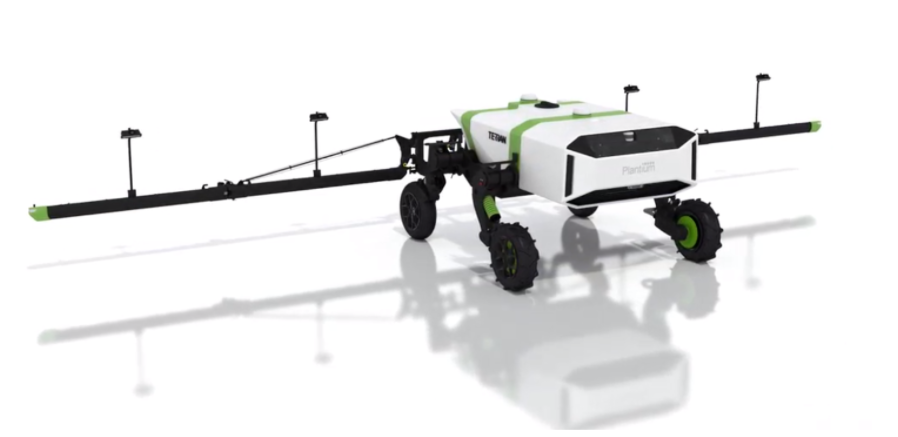
\includegraphics[width=.8\textwidth]{./Figuras/terran_3d.png}
\caption{Modelo 3D de Terran}
\label{fig:terran_3d}
\end{figure}

Actualmente, existe construido un prototipo que cuenta con un sistema de navegación y control que le permite circular de manera autónoma sobre trayectorias predefinidas. Además, el módulo responsable de aplicación selectiva se encuentra en funcionamiento. Sin embargo, no hay implementado ningún mecanismo inteligente para detectar, reconocer y esquivar obstáculos y evitar así posibles colisiones.

Con este fin, Terran cuenta con un sensor LiDAR integrado en la placa de desarrollo que se comunica con los demás módulos del vehículo. Haciendo uso de este sensor, el vehículo es capaz de detectar objetos y detenerse para evitar la colisión. Si posteriormente el obstáculo es removido, se envía una señal de avance al módulo de control y continúa la circulación sobre la trayectoria definida.

Por otro lado, la lógica de detección de obstáculos actualmente implementada no se basa en un algoritmo inteligente. Para definir si un objeto es o no un obstáculo, la nube de puntos generada por el sensor LiDAR es procesada y dividida en dos partes mediante una línea horizontal u “horizonte”. Todos los puntos que se encuentren en la parte inferior de esta división son descartados y no son tenidos en cuenta en la detección de objetos. Por el contrario, cualquier conjunto de puntos que se encuentre por encima de este horizonte es considerado un obstáculo, y obligará al vehículo a detenerse. 

Es evidente que este sistema no cuenta con la robustez necesaria para realizar una  navegación autónoma satisfactoria. Se ha comprobado que el vehículo no logra diferenciar correctamente entre personas, nubes de polvo o yuyos y malezas de gran altura. Además, será necesario realizar la detección de pozos y zanjones, haciendo uso de los puntos inferiores descartados o  de los datos provenientes de nuevos sensores.

En este contexto surge la necesidad de dotar de inteligencia al sistema de navegación del vehículo, lo que plantea dos desafíos:

\begin{itemize}
\item El primero es la integración de sensores para poder lograr un mapeo completo del terreno en 360 grados y en diferentes condiciones climáticas. Esto implica embeber los sensores al hardware desarrollado y lograr la recolección de los datos. El conjunto de sensores propuesto está formado por:
\begin{itemize}
\item LiDAR (ya instalado)
\item Cámaras 
\item Radar
\end{itemize}
\item La segunda etapa es la de procesar los datos obtenidos y aplicar técnicas de inteligencia artificial que permitan la correcta detección de obstáculos y la estimación de las condiciones del terreno para proceder con el cálculo de una nueva trayectoria. En este sentido, existen dos grandes conjuntos de tareas que deben ser implementadas:
\begin{itemize}
\item El procesamiento de imágenes capturadas por las cámaras para poder realizar la detección de obstáculos y eventualmente de pozos y zanjones.
\item La fusión de los datos proveniente de los sensores, con el fin de utilizar esta información de manera conjunta y lograr mejores resultados al momen o de tomar decisiones en la navegación.
\end{itemize}
\end{itemize}

Es dentro del marco de ejecución de esta segunda etapa en donde se desarrollará el proyecto propuesto en el actual documento. Particularmente, se realizarán las tareas relacionadas al procesamiento de las imágenes capturadas por las cámaras a partir de la aplicación de técnicas de visión artificial. En términos generales, el objetivo será lograr detectar pozos y charcos y localizar surcos, haciendo uso de las imágenes de las cámaras. Los resultados de este proceso, combinados con el procesamiento de datos de los demás sensores, permitirá mejorar la toma de decisiones en la navegación y calcular nuevas trayectorias para evitar posibles colisiones con obstáculos.

En la Figura \ref{fig:diagBloques} se presenta el diagrama de bloques del sistema. Se observa que los datos crudos obtenidos por el conjunto de sensores (cámaras, LiDAR y radar) son procesados de manera independiente con el objetivo de mejorar la calidad de los datos. En esta etapa se debe identificar y eliminar datos que pueden considerarse ruido, rellenar valores faltantes, resolver redundancia y corregir inconsistencias.

Los datos del LiDAR y radar son combinados en una segunda etapa donde se aplican técnicas de fusión de datos (\emph{sensor fusion}). Los datos provenientes de las cámaras son procesados de manera independiente para detectar los objetos mencionados. Los resultados son enviados a un sistema encargado de tomar decisiones basadas en los datos informados por los sensores. En base a esto, el módulo de navegación realiza el cálculo de las trayectorias y las envía al sistema de control responsable del movimiento del vehículo. Esta etapa de navegación y control se encuentra actualmente implementada.

La línea de trazos naranja en el diagrama de bloque muestra las etapas implicadas en el proyecto actual. Así, el siguiente proyecto se desarrollará sobre las etapas de recolección y procesamiento de datos de las cámaras.


\begin{figure}[htpb]
\centering 
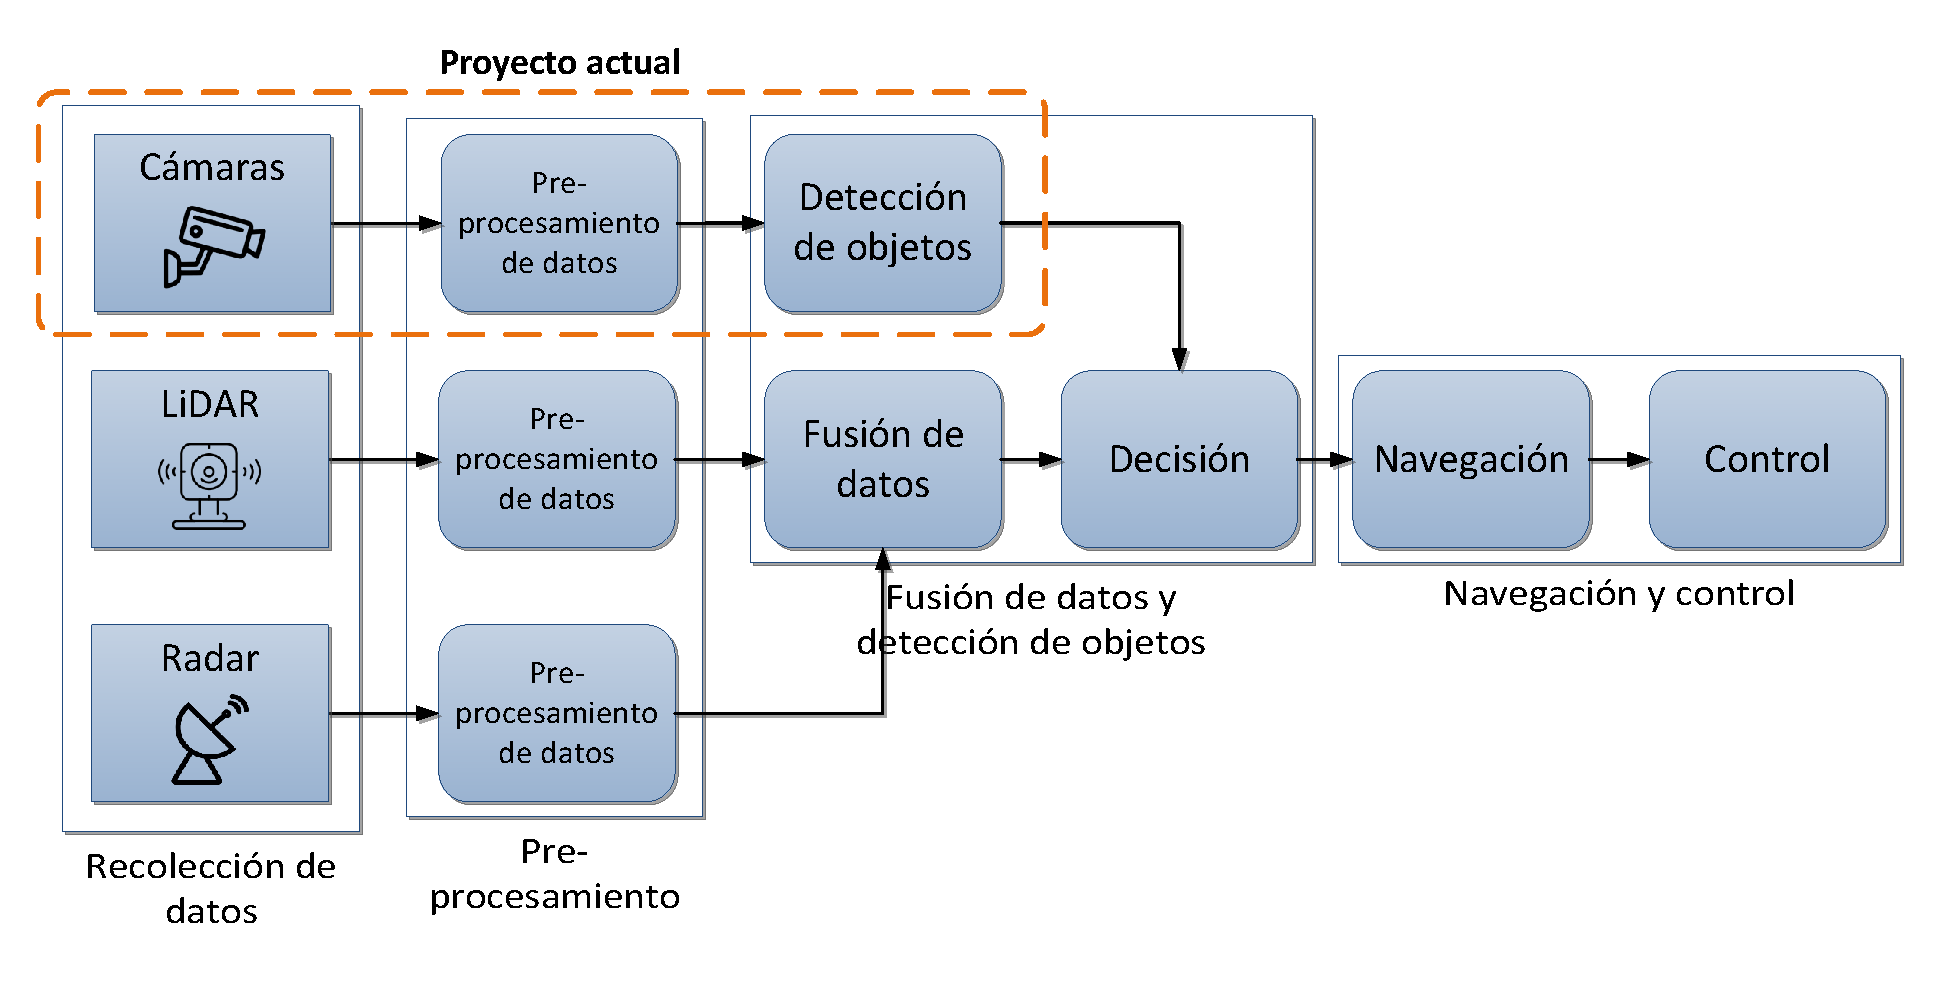
\includegraphics[width=1\textwidth]{./Figuras/diagBloques.pdf}
\caption{Diagrama de bloques del sistema}
\label{fig:diagBloques}
\end{figure}

\section{2. Identificación y análisis de los interesados}
\label{sec:interesados}

\begin{table}[ht]
%\caption{Identificación de los interesados}
%\label{tab:interesados}
\begin{tabularx}{\linewidth}{@{}|l|X|X|X|@{}}
\hline
\rowcolor[HTML]{C0C0C0} 
Rol           & Nombre y Apellido & Organización 	& Puesto 					\\ \hline
Cliente       & \clientename      &\empclientename	& Project manager 			\\ \hline
Responsable   & \authorname       & FIUBA        	& Alumno 					\\ \hline
Orientador    & \supname	      & \pertesupname 	& Director trabajo final 	\\ \hline
Equipo        & Andres Benso \newline Mateo Cervilla 
			  & Plantium S.A. \newline Plantium S.A. 
			  & Team Leader \newline Software Developer \\ \hline
Opositores    & Empresas competidoras orientadas a la robótica para el agro&  - &- \\ \hline
Usuario final &  Productores agropecuarios  &      -     	&    -    			\\ \hline
\end{tabularx}
\end{table}

\section{3. Propósito del proyecto}
\label{sec:proposito}

El propósito de este proyecto es desarrollar un sistema de visión artificial que formará parte de un sistema de navegación inteligente en parcelas agrícolas, destinado a detectar obstáculos y estimar las condiciones del terreno. Estas estimaciones se utilizarán para mejorar la toma de decisiones en la navegación mediante el cálculo de nuevas trayectorias que eviten posibles colisiones con los distintos obstáculos. En una etapa posterior, el sistema inteligente se integrará con los módulos de navegación existentes con el objetivo de lograr un vehículo completamente autónomo capaz de realizar la pulverización selectiva en los terrenos.

\section{4. Alcance del proyecto}
\label{sec:alcance}

Si bien la etapa de adquisición y procesamiento de datos del proyecto Terran incluye una gran cantidad de actividades, el alcance del presente proyecto se limita a cumplir los siguientes objetivos y tareas:

\begin{itemize}
	\item Correcta detección en tiempo real de surcos, utilizando los datos de las cámaras.
	\item Investigar metodologías y tecnologías a utilizar relacionadas al procesamiento de imágenes (algoritmos, bibliotecas, frameworks, etc.).
	\item Creación de datasets necesarios para entrenar y evaluar los modelos utilizados. 
\end{itemize}

Adicionalmente, en el transcurso del proyecto se evaluará la posibilidad de incluir la detección en tiempo real de pozos y charcos, utilizando los datos de las cámaras.

Por otra parte, no se consideran incluidas en este proyecto las tareas relacionadas con:

\begin{itemize}
	\item Integración de sensores al hardware.
	\item Procesamiento de datos del LiDAR o radar.	
	\item Integración de datos provenientes de los distintos sensores.
	\item Implementación de la comunicación de los sensores con el módulo de procesamiento de datos. Tampoco se incluirá la comunicación entre este último módulo y el sistema de navegación.
	\item Cálculo de nuevas trayectorias.
	\item Tareas relacionadas a la navegación, control y seguimiento de trayectoria.
\end{itemize}

\section{5. Supuestos del proyecto}
\label{sec:supuestos}

Para el desarrollo del presente proyecto se supone que:

\begin{itemize}
	\item La etapa previa que incluye la integración de sensores al hardware se encuentra implementada y en correcto funcionamiento.
	\item Se cuenta con el hardware necesario para la realización del proyecto. Esto incluye:
\begin{itemize}
	\item Servidor para almacenar y procesar datos.
	\item Cámaras.
\end{itemize}
	\item Tanto el hardware como las licencias de software que se necesiten serán adquiridos sin inconvenientes, siendo la empresa quien cubra los gastos que surjan en esos casos.
	
\end{itemize}

\section{6. Requerimientos}
\label{sec:requerimientos}

\begin{enumerate}
	\item Requerimientos funcionales
		\begin{enumerate}
			\item El sistema debe poder detectar surcos con un error menor al 10\%, en buenas condiciones de iluminación.
			\item La salida del sistema debe ser una variable que indique la posición relativa en la imagen de los surcos detectados.
			\item El sistema debe poder operar en tiempo real (prioridad menor).
		\end{enumerate}
		
	\item Requerimientos opcionales
		\begin{enumerate}
			\item El sistema debe poder detectar pozos y charcos con un error menor al 10\%, en buenas condiciones de iluminación.
			\item La salida del sistema debe ser una variable que informe si existe o no un pozo en el camino.
		\end{enumerate}
	
	\item Requerimientos de documentación
		\begin{enumerate}
			\item Los códigos desarrollados deben estar documentados según buenas prácticas sugeridas por el cliente. Esta documentación debe permitir que el código pueda ser entendido y utilizado por cualquier otro miembro de la empresa, con los conocimientos técnicos necesarios.
			\item Confección de una memoria técnica.
			\item Confección de un manual de uso.
		\end{enumerate}
	\item Requerimientos de testeo
		\begin{enumerate}
			\item Debe probarse la efectividad del sistema en terrenos agropecuarios y en distintas condiciones ambientales y de iluminación.
		\end{enumerate}
\end{enumerate}


\section{7. Historias de usuarios (\textit{Product backlog})}
\label{sec:backlog}

Los criterios para el cálculo de las ponderaciones (\textit{history points}) de las historias de usuarios son los siguientes:

\begin{itemize}
	\item Dificultad: es la cantidad de trabajo a realizar. Involucra el total de horas y recursos empleados en la tarea.
	\item Complejidad: es el nivel de sofisticación del trabajo. Hace referencia al nivel de conocimientos o habilidades requeridos para realizar la tarea.
	\item Riesgo: es el nivel de incertidumbre que involucra realizar la tarea.
\end{itemize}

A cada criterio se le asigna un peso que se corresponden con los números del 1 al 13 de la serie de Fibonacci (1, 2, 3, 5, 8, 13). El peso total de la historia de usuario será el número de la serie de Fibonacci más cercano a la suma de los pesos de cada criterio.

Historia 1: ''Como usuario final quiero que el vehículo pueda funcionar de noche para poder trabajar el terreno las 24hs."

\begin{itemize}
	\item Dificultad: 5. Se requieren horas de investigación para mejorar la calidad de los datos de noche.
	\item Complejidad: 13. La confiabilidad de las cámaras es baja a la noche. Su utilidad depende completamente de la iluminación provista por el vehículo.
	\item Riesgo: 1. No existen mayores riesgos a excepción de la pérdida de precisión en la clasificación de obstáculos en estas condiciones.
\end{itemize}

Peso total: 21

Historia 2: ''Como gerente técnico quiero que el sistema sea fácilmente reentrenable para poder mejorar la precisión con datos futuros."

\begin{itemize}
	\item Dificultad: 5. No afecta demasiado al diseño pero se requiere asignar tiempo para documentación en manuales y códigos.
	\item Complejidad: 2. La complejidad es baja y radica en diseñar las entradas del modelo de manera amigable.
	\item Riesgo: 3. Modificar el modelo podría llegar a impactar en la precisión de manera negativa. Sin embargo, es fácil volver a modelos previos en caso de que ocurra este inconveniente.
\end{itemize}
	
Peso total: 8

Historia 3: ''Como empresa me interesa que el sistema pueda reconocer tambíen vehículos para futuras aplicaciones"

\begin{itemize}
	\item Dificultad: 13. Se deberá dedicar mucho tiempo al armado de datasets que contengan distintos vehículos.
	\item Complejidad: 2. El proceso de entrenamiento y el modelo a utilizar no se afectan demasiado.
	\item Riesgo: 3. Agregar nuevas clases puede afectar a la eficiencia del modelo sobre las predicciones de las clases originales.
\end{itemize}
	
Peso total: 21

\section{8. Entregables principales del proyecto}
\label{sec:entregables}

Los entregables del proyecto son:

\begin{itemize}
	\item Código fuente
	\item Dataset con datos originales
	\item Dataset con datos pre-procesados.
	\item Memoria técnica.
	\item Documentación de uso del modelo.
\end{itemize}


\section{9. Desglose del trabajo en tareas (WBS)}
\label{sec:wbs}

\begin{enumerate}
	\item \textbf{Gestión de proyecto (20hs)}
	\begin{enumerate}
		\item Desarrollo de plan de trabajo (20hs)
	\end{enumerate}

\item \textbf{Investigación previa (80hs)}
	\begin{enumerate}
		\item Investigación sobre trabajos similares (20hs)
		\item Investigación de técnicas para preprocesado de imágenes (20hs)
		\item Investigación sobre modelos existentes y pre-entrenados (20hs)
		\item Investigación sobre tecnicas de seguimiento sobre imágenes (20hs)
	\end{enumerate}

\item \textbf{Generación de dataset (90hs)}
	\begin{enumerate}
		\item Búsqueda de datasets existentes (10hs)
		\item Definición de buenas prácticas para la generación de datasets (10hs)
		\item Recolección de datos con las cámaras (40hs)
		\item Etiquetado de datos (30hs)
	\end{enumerate}

\item \textbf{Preprocesado (40hs)}
	\begin{enumerate}
		\item Diseño e implementación de pipeline para preprocesado de imágenes (40hs)
	\end{enumerate}

\item \textbf{Generación del modelo (190hs)}
	\begin{enumerate}
		\item Creación de diferentes prototipos de modelos (30hs)
		\item Evaluación de desempeño de prototipos y selección de modelo a utilizar (15hs)
		\item Perfeccionamiento del modelo utilizando dataset original (40hs)
		\item Diseño e implementación de pipeline para seguimiento de surcos (30hs)
		\item Ajuste de modelo posterior a las pruebas en simulación (30hs)
		\item Ajuste de modelo posterior a las pruebas en campo (30hs)
		\item Documentación del código (15hs)
	\end{enumerate}

\item \textbf{Testeo y evaluación (120hs)}
	\begin{enumerate}
		\item Investigación y definición de criterios de evaluación del modelo (10hs)
		\item Diseño de casos de prueba y tests a realizar (10hs)
		\item Preparación de entorno de simulación (20hs)
		\item Testeo de modelo en entorno de simulación (25hs)
		\item Testeo de modelo en campo (30hs)
		\item Pruebas finales del modelo (15hs)
		\item Documentación de pruebas (10hs)
	\end{enumerate}

\item \textbf{Documentos finales (70hs)}
	\begin{enumerate}
		\item Confección de manual de uso de modelo (15hs)
		\item Confección del informe de avance (10hs)
		\item Confección de la memoria del trabajo (30hs)
		\item Preparación de la presentación final (15hs)
	\end{enumerate}
	
\end{enumerate}


Cantidad total de horas: 610hs


\section{10. Diagrama de Activity On Node}
\label{sec:AoN}

En la figura \ref{fig:aon} se muestra el diagrama en Activity on Node (AoN) del proyecto. Los períodos de tiempo (t) están expresados en días. Para el cálculo, se establecieron 12hs de trabajo semanales, divididas en 4 días de 3hs cada uno. Los bloques color salmón indican la ruta crítica.

Con el fin de mantener una lógica sencilla en el diagrama AoN, las tareas del WBS fueron agrupadas en diferentes bloques, tal como se indica en la siguiente lista:

\begin{itemize}

\item \textbf{Planificacion (t=7)}:
\begin{itemize}
\item 1.1. Desarrollo de plan de trabajo
\end{itemize}

\item \textbf{Investigación previa (t=20)}:
\begin{itemize}
\item 2.1. Investigación sobre trabajos similares
\item 2.2. Investigación de técnicas para preprocesado de imágenes
\item 2.3. Investigación sobre modelos existentes y pre-entrenados
\end{itemize}

\item \textbf{Armado de datset (t=30)}:
\begin{itemize}
\item 3.1. Búsqueda de datasets existentes
\item 3.2. Definición de buenas prácticas para la generación de datasets
\item 3.3. Recolección de datos con las cámaras
\item 3.4. Etiquetado de datos
\end{itemize}

\item \textbf{Investigación sobre técnicas de seguimiento (t=7)}:
\begin{itemize}
\item 2.4. Investigación sobre tecnicas de seguimiento sobre imágenes
\end{itemize}

\item \textbf{Pipeline para preprocesado de imagenes (t=13)}:
\begin{itemize}
\item 4.1. Dise˜no e implementación de pipeline para preprocesado de imágenes
\end{itemize}

\item \textbf{Pipeline para seguimiento de surcos (t=10)}:
\begin{itemize}
\item 5.4. Dise˜no e implementación de pipeline para seguimiento de surcos
\end{itemize}

\item \textbf{Selección de modelo a preeliminar (t=28)}:
\begin{itemize}
\item 5.1. Creación de diferentes prototipos de modelos
\item 5.2. Evaluación de desempe˜no de prototipos y selección de modelo a utilizar
\item 5.3. Perfeccionamiento del modelo utilizando dataset original
\end{itemize}

\item \textbf{Investigación y diseño de tests (t=7)}:
\begin{itemize}
\item 6.1. Investigación y definición de criterios de evaluación del modelo
\item 6.2. Dise˜no de casos de prueba y tests a realizar
\end{itemize}

\item \textbf{Testeo y ajuste del modelo en simulación (t=25)}:
\begin{itemize}
\item 6.3. Preparación de entorno de simulación
\item 6.4. Testeo de modelo en entorno de simulación
\item 5.5. Ajuste de modelo posterior a las pruebas en simulación
\end{itemize}

\item \textbf{Confección de informe de avance (t=3)}:
\begin{itemize}
\item 7.2. Confección del informe de avance
\end{itemize}

\item \textbf{Testeo y ajuste del modelo en campo (t=20)}:
\begin{itemize}
\item 6.5. Testeo de modelo en campo
\item 5.6. Ajuste de modelo posterior a las pruebas en campo
\end{itemize}

\item \textbf{Pruebas finales (t=5)}:
\begin{itemize}
\item 6.6. Pruebas finales del modelo
\end{itemize}

\item \textbf{Documentación de código (t=5)}:
\begin{itemize}
\item 5.7. Documentación del código
\end{itemize}

\item \textbf{Documentación de pruebas (t=3)}:
\begin{itemize}
\item 6.7. Documentación de pruebas
\end{itemize}

\item \textbf{Documentación final (t=20)}:
\begin{itemize}
\item 7.1. Confección de manual de uso de modelo
\item 7.3. Confección de la memoria del trabajo
\item 7.4. Preparación de la presentación final
\end{itemize}

\end{itemize}

\begin{figure}[htpb]
\centering 
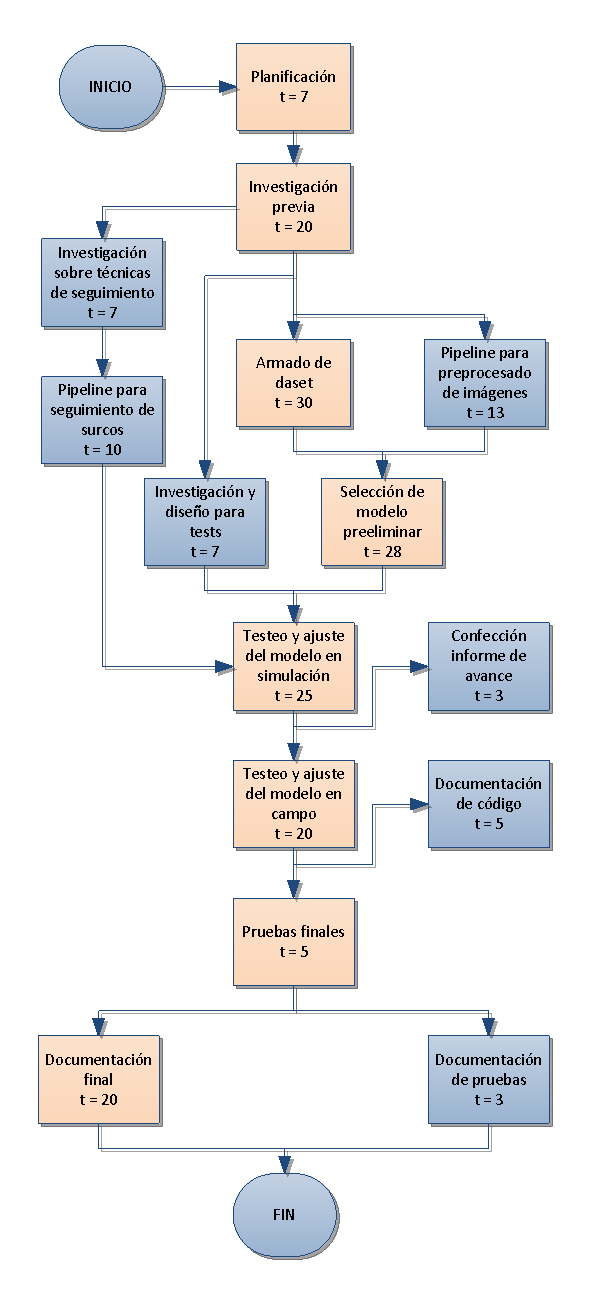
\includegraphics[width=.65\textwidth]{./Figuras/aon.pdf}
\caption{Diagrama en \textit{Activity on Node}}
\label{fig:aon}
\end{figure}


\section{11. Diagrama de Gantt}
\label{sec:gantt}

La figura \ref{fig:gantt_tabla} muestra la tabla con las tareas representadas en el diagrama de Gantt, en donde se incluyen los códigos del WBS. En la figura \ref{fig:diagGantt} se muestra el diagrama de Gantt. El camino crítico está representado por las tareas rayadas en color más oscuro.

\begin{figure}[htpb]
\centering 
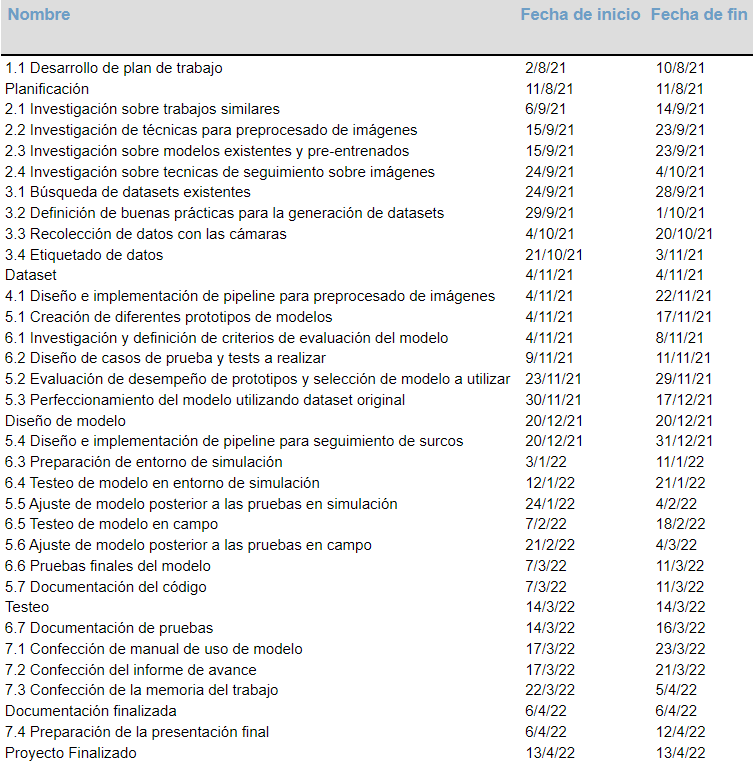
\includegraphics[width=1\textwidth]{./Figuras/gantt_tabla.png}
\caption{Tabla de WBS}
\label{fig:gantt_tabla}
\end{figure}


\begin{landscape}
\begin{figure}[htpb]
\centering 
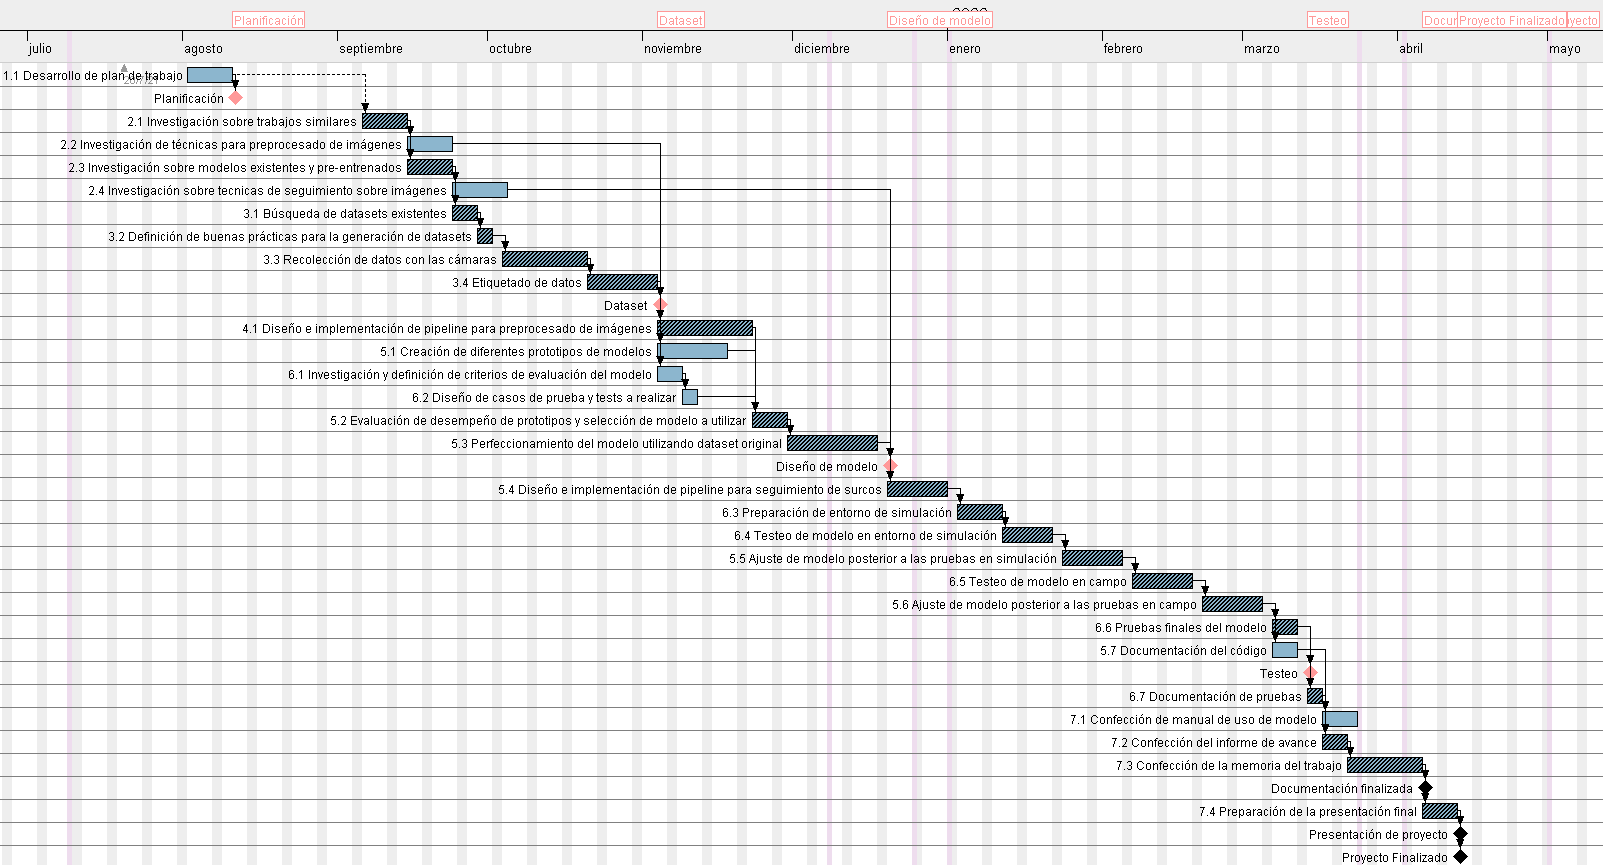
\includegraphics[height=.85\textheight]{./Figuras/gantt.png}
\caption{Diagrama de Gantt}
\label{fig:diagGantt}
\end{figure}
\end{landscape}



\section{12. Presupuesto detallado del proyecto}
\label{sec:presupuesto}

\begin{table}[htpb]
\centering
\begin{tabularx}{\linewidth}{@{}|X|c|r|r|@{}}
\hline
\rowcolor[HTML]{C0C0C0} 
\multicolumn{4}{|c|}{\cellcolor[HTML]{C0C0C0}COSTOS DIRECTOS} \\ \hline
\rowcolor[HTML]{C0C0C0} 
Descripción &
  \multicolumn{1}{c|}{\cellcolor[HTML]{C0C0C0}Cantidad} &
  \multicolumn{1}{c|}{\cellcolor[HTML]{C0C0C0}Valor unitario [\$]} &
  \multicolumn{1}{c|}{\cellcolor[HTML]{C0C0C0}Valor total [\$]} \\ \hline
Horas del responsable &
  \multicolumn{1}{c|}{610} &
  \multicolumn{1}{c|}{750} &
  \multicolumn{1}{c|}{457.500} \\ \hline
Notebook &
  \multicolumn{1}{c|}{1} &
  \multicolumn{1}{c|}{350.000} &
  \multicolumn{1}{c|}{350.000} \\ \hline
Licencia Simulador &
  \multicolumn{1}{c|}{1} &
  \multicolumn{1}{c|}{200.000} &
  \multicolumn{1}{c|}{200.000} \\ \hline
\multicolumn{3}{|c|}{SUBTOTAL} &
  \multicolumn{1}{c|}{1.007.500} \\ \hline
\rowcolor[HTML]{C0C0C0} 
\multicolumn{4}{|c|}{\cellcolor[HTML]{C0C0C0}COSTOS INDIRECTOS} \\ \hline
\rowcolor[HTML]{C0C0C0} 
Descripción &
  \multicolumn{1}{c|}{\cellcolor[HTML]{C0C0C0}Cantidad} &
  \multicolumn{1}{c|}{\cellcolor[HTML]{C0C0C0}Valor unitario [\$]} &
  \multicolumn{1}{c|}{\cellcolor[HTML]{C0C0C0}Valor total [\$]} \\ \hline
Transporte para pruebas en campo &
  \multicolumn{1}{c|}{1} &
  \multicolumn{1}{c|}{30.000} &
  \multicolumn{1}{c|}{30.000} \\ \hline
Gastos mensuales de oficina &
  \multicolumn{1}{c|}{9} &
  \multicolumn{1}{c|}{5.000} &
  \multicolumn{1}{c|}{45.000} \\ \hline
\multicolumn{3}{|c|}{SUBTOTAL} &
  \multicolumn{1}{c|}{120.000} \\ \hline
\rowcolor[HTML]{C0C0C0}
\multicolumn{3}{|c|}{TOTAL} & 1.127.500 [\$]
   \\ \hline
\end{tabularx}%
\end{table}


\section{13. Gestión de riesgos}
\label{sec:riesgos}

Los riesgos identificados en esta sección son cuantificados mediante los siguientes indicadores:

\begin{itemize}
    \item Severidad (S): índice de severidad. Será mayor cuanto más grande sea el impacto sobre el proyecto.
    \item Ocurrencia (O): probabilidad de ocurrencia del riesgo.
\end{itemize}
	
A cada uno de estos índices se le asigna un valor del 1 al 10. El número que resulta del producto de ambos es la prioridad del riesgo (RPN = S*O).

Los riesgos identificados asociados al proyecto son:

\begin{itemize}
	\item Riesgo 1: la etapa previa de incorporación de las cámaras al hardware toma más tiempo del estimado.
	\begin{itemize}
		\item Severidad (7): atrasaría el inicio del proyecto y alteraría la gestión de tiempo.
		\item Ocurrencia (5): dado que las cámaras a utilizar aún no están definidas, podían surgir inconveniente por compatibilidades que produzcan la extensión de los plazos de esta etapa. 
	\end{itemize}
	
	\item Riesgo 2: escasez de información sobre temas a investigar.
	\begin{itemize}
		\item Severidad (6): complicaría el desarrollo general del proyecto. Podría producir un gasto adicional de tiempo para pruebas de diferentes técnicas y enfoques que sean poco eficientes.
		\item Ocurrencia (3): si bien es probable que no haya demasiada información sobre trabajos idénticos al que se desarrollará en este proyecto, existe mucha información sobre trabajos similares de navegación autónoma que pueden ser adaptados al entorno agropecuario.
	\end{itemize}
	
	\item Riesgo 3: la capacidad del hardware actual no es suficiente para realizar el procesamiento de imágenes en tiempo real.
	\begin{itemize}
		\item Severidad (6): no se podrá realizar la detección en tiempo real.
		\item Ocurrencia (5): no se ha probado el hardware en aplicaciones de procesamiento de imágenes.
	\end{itemize}
	
	\item Riesgo 4: que exista mucha discrepancia entre los resultados de las pruebas de simulación y su uso en el campo.
	\begin{itemize}
		\item Severidad (3): se ha considerado esta dificultad dentro de las horas asignadas a las tareas correspondientes. 
		\item Ocurrencia (8): dado que la cantidad de simuladores para terrenos agropecuarios es limitada, será difícil encontrar un simulador con una alta fidelidad en los datos proporcionados.
	\end{itemize}
	
	\item Riesgo 5: licencias más caras de lo planificado.
	\begin{itemize}
		\item Severidad (6): podría producir que los costos del proyecto superen a lo planificado.
		\item Ocurrencia (3): se han verificado precios de posibles licencias antes de realizar la gestión de costos.
	\end{itemize}
	
	\item Riesgo 6: falla en base de datos donde se almacena el dataset creado.
	\begin{itemize}
		\item Severidad (10): el rearmado del dataset produciría un gran retraso en el proyecto.
		\item Ocurrencia (4): está contemplado realizar backups del dataset.
	\end{itemize}

\end{itemize}
	
La siguiente tabla muestra los riesgos listados anteriormente, con sus correspondientes prioridades (RPN). Los valores marcados con (*) indican los resultados luego de haber aplicado la mitigación.

\begin{table}[htpb]
\centering
\begin{tabularx}{\linewidth}{@{}|X|c|c|c|c|c|c|@{}}
\hline
\rowcolor[HTML]{C0C0C0} 
Riesgo 						  & S  & O & RPN & S* & O* & RPN*	\\ \hline
1.- Retrasos en etapa previa  & 7  & 5 & 35  & 2 & 5 & 10		\\ \hline
2.- Falta de información 	  & 6  & 3 & 18  &   &   &		\\ \hline
3.- Hardware limitado 		  & 6  & 5 & 30  & 1 & 5 & 5 	\\ \hline
4.- Simulación poco eficiente & 3  & 8 & 24  &   &   &  	\\ \hline
5.- Licencias caras			  & 6  & 3 & 18  &   &   &  	\\ \hline
6.- Pérdida de dataset		  & 10 & 4 & 40  & 2 & 1 & 2  	\\ \hline
\end{tabularx}%
\end{table}

Se tomarán medidas de mitigación en los riesgos cuyos números de RPN sean mayores a 25. El plan de mitigación de riesgo, se detalla a continuación:

\begin{itemize}

	\item Riesgo 1: en el AON puede verse que en la primer parte del proyecto la mayoría de las tareas tienen holgura, a excepción de las que forman parte del camino crítico. Particularmente este riesgo podría afectar en la demora del armado del dataset. Por este lado, se plantea que la recolección de datos se realice con otro juego de cámaras, similares a las integradas al hardware. La siguiente tarea del camino crítico que podría afectarse son las pruebas del modelo en campo. Sin embargo, en base al el diagrama de Gannt, esta tarea forma parte de una de las últimas del proyecto, por lo que es muy poco probable que sea afectada por el riesgo en cuestión.
	\begin{itemize}
		\item Severidad (2): al usar otro juego de cámaras, la primer parte del proyecto no se verá afectada por posibles demoras en la etapa previa.
		\item Ocurrencia (5): no se ha modificado al probabilidad de ocurrencia.
	\end{itemize}
	
	\item Riesgo 3: dado que el alcance y los requisitos del proyecto propuestos consisten en la entrega de un algoritmo, no es necesario realizar las pruebas sobre el hardware final. Por lo tanto, en caso que ocurra este riesgo, las pruebas en campo serán realizadas utilizando las cámaras montadas sobre el vehículo, conectadas a la notebook de desarrollo que realizará el procesamiento de imágenes.
	\begin{itemize}
		\item Severidad (1): utilizando otro hardware alternativo, el proyecto no se verá afectado por limitaciones en el hardware.
		\item Ocurrencia (5): no se ha modificado al probabilidad de ocurrencia.
	\end{itemize}
	
	\item Riesgo 6: se realizará un backup periódico en la nube del estado actual del dataset.
	\begin{itemize}
		\item Severidad (2): como los backups son realizados de manera periódica, cualquier problema que ocurra en la base de datos sólo afectara el trabajo de un día.
		\item Ocurrencia (1): es muy poco probable perder los datos en los servidores locales y en la nube al mismo tiempo.
	\end{itemize}
\end{itemize}



\section{14. Gestión de la calidad}
\label{sec:calidad}

\begin{itemize}
	
	\item Req 1.1: el sistema debe poder detectar surcos con un error menor al 10\%, en buenas condiciones de iluminación.
	\begin{itemize}
		\item Verificación: en el entorno de simulación, debe simularse el vehículo conduciendo sobre diferentes surcos en un día soleado. La prueba total debe durar al menos 20 minutos. Durante toda la prueba, el vehículo debe ser capaz de detectar el surco por el que conduce por más del 90\% del tiempo.
		\item Validación: se procesarán videos grabados por el vehículo conduciendo sobre diferentes surcos en un día soleado. La duración total de los videos, debe ser de al menos 20 minutos. Procesando las imágenes de las grabaciones, deben poder detectarse los surcos por los que se esté conduciendo al menos el 90\% del tiempo.
	\end{itemize}
	\item Req 1.2: la salida del sistema debe ser una variable que indique la posición relativa en la imagen de los surcos detectados.
	\begin{itemize}
		\item Verificación: en las grabaciones de las simulaciones, se debe marcar con una máscara de cuatro vértices la posición del surco en la imagen. Además, debe generarse un archivo de log que indique las posiciones en píxeles de los cuatro vértices de la máscara en cada frame.
		\item Validación: en las grabaciones realizadas en campo, se debe marcar con una máscara de cuatro vértices la posición del surco en la imagen. Además, debe generarse un archivo de log que indique las posiciones en píxeles de los cuatro vértices de la máscara en cada frame.
	\end{itemize}
	\item Req 1.3: el sistema debe poder operar en tiempo real (prioridad menor).
	\begin{itemize}
		\item Verificación: debe probarse en entorno de simulación. La variable binaria de salida que indica la detección de pozos y charcos debe poder visualizarse y activarse correctamente en tiempo real, mientras se conduce en simulación. De igual manera, las imágenes capturadas por las cámaras en la simulación, deben ser mostradas en tiempo real, con la máscara de cuatro vértices aplicada sobre los surcos.
		\item Validación: debe probarse con el vehículo en campo. La variable binaria de salida que indica la detección de pozos y charcos debe poder visualizarse y activarse correctamente en tiempo real. De igual manera, las imágenes capturadas por las cámaras, deben ser mostradas en tiempo real, con la máscara de cuatro vértices aplicada sobre los surcos.
	\end{itemize}
	\item Req 2.1: el sistema debe poder detectar pozos y charcos con un error menor al 10\%, en buenas condiciones de iluminación.
	\begin{itemize}
		\item Verificación: en el entorno de simulación, debe simularse el vehículo y una cantidad no menor a 30 pozos y/o charcos en un día soleado. El vehículo debe ser capaz de detectar al menos un 90\% de esos pozos y charcos.
		\item Validación: se procesarán videos grabados por el vehículo en el campo en un día soleado, en donde deben aparecer una cantidad no menor a 20 pozos y/o charcos. Procesando las imágenes de los videos, deben poder detectarse al menos el 90\% de esos pozos.
	\end{itemize}
	\item Req 2.2: la salida del sistema debe ser una variable que informe si existe o no un pozo en el camino.
	\begin{itemize}
		\item Verificación: se graficará la salida binaria del sistema en función del tiempo y se evaluará la correlación entre sus valores con las grabaciones de la simulación. La gráfica debe mostrar un valor igual a 1 en los momentos en que en las grabaciones se visualicen pozos o charcos.
		\item Validación: se graficará la salida binaria del sistema en función del tiempo y se evaluará la correlación entre sus valores con las grabaciones en el campo. La gráfica debe mostrar un valor igual a 1 en los momentos en que en las grabaciones se visualicen pozos o charcos.
	\end{itemize}
	\item Req 3.1: los códigos desarrollados deben estar documentados según buenas prácticas sugeridas por el cliente. Esta documentación debe permitir que el código pueda ser entendido y utilizado por cualquier otro miembro de la empresa, con los conocimientos técnicos necesarios.
	\begin{itemize}
		\item Verificación: el team leader revisará los códigos desarrollados y verificará su correcta documentación. Debe ser capaz de entender en detalle cada proceso o función desarrollada.
		\item Validación: un miembro de la empresa con los conocimientos técnicos necesarios, ajeno a los integrantes del proyecto, revisará los códigos desarrollados y verificará su correcta documentación. Debe ser capaz de comprender cuáles son las entradas y salidas de los distintos módulos del sistema.
	\end{itemize}
	\item Req 3.2: confección de una memoria técnica.
	\begin{itemize}
		\item Verificación: La memoria técnica debe ser aprobada por el director y el project manager del proyecto, que definirán sus propios criterios de validación. 
		\item Validación: La memoria técnica debe ser aprobada por los docentes y jurados de la FIUBA, que definirán sus propios criterios de validación.
	\end{itemize}
	\item Req 3.3: confección de un manual de uso.
	\begin{itemize}
		\item Verificación: el team leader verificará que todos los submódulos del sistema se encuentren documentados, explicitando su función y sus entradas y salidas. Por otro lado, debe estar documentado el proceso de instalación y puesta en marcha. El team leader deberá ser capaz de poner en marcha y utilizar el sistema completo, a partir del manual de usuario.
		\item Validación: el project manager deberá verificar y aprobar la calidad del manual de usuario.
	\end{itemize}
	\item Req 4.1: debe probarse la efectividad del sistema en terrenos agropecuarios y en distintas condiciones ambientales y de iluminación.
	\begin{itemize}
		\item Verificación: se realizará la misma verificación que en los requerimientos 1.1 y 1.2 con un entorno de simulación de un día nublado. La precisión lograda en ambos casos, debe ser superior al 75\%. 
		\item Validación: se realizará la misma validación que en los requerimientos 1.1 y 1.2, con grabaciones en campo de días nublados. La precisión lograda en ambos casos, debe ser superior al 75\%.
	\end{itemize}
\end{itemize} 

\section{15. Procesos de cierre}    
\label{sec:cierre}

El proceso de cierre consiste en las siguientes actividades:

\begin{itemize}
\item Verificación del cumplimiento de objetivos: deberá comprobarse que todos los objetivos fueron alcanzados. Para esto se debe demostrar que todos los requerimientos cumplieron con los criterios de verificación y validación escritos en el apartado ''14. Gestión de la calidad'' del plan de trabajo. Además, deberá verificarse la correcta recepción de todos los entregables.

Reponsable: Ariel G. Moreno (project manager)


\item Análisis del grado de cumplimiento del plan de proyecto:

\begin{itemize}
\item  Gestión de tiempo: identificar discrepancias entre las tareas planteadas en el WBS y su estimación de tiempo en el diagrama de Gannt con las tareas y los tiempos de ejecución reales.
\item  Gestión de costos: verificar si existe diferencia entre el costo del proyecto estimado con el real.
\end{itemize}

Responsable: Agustin Baffo (responsable del proyecto)

\item Memoria de problemas encontrados y técnicas utilizadas:
deberán identificarse y documentarse los problemas que hayan surgido, así como también las soluciones planteadas incluyendo tanto las finales como las que hayan fracasado.

Responsable: Agustin Baffo (responsable del proyecto)


\item Memoria de técnicas y enfoques utilizados: se identificarán y documentarán técnicas y enfoques que hayan sido exitosos para asegurarse que su uso será considerado en el futuro. De igual forma, se documentarán técnicas y enfoques que hayan fracasado para asegurarse que serán descartados en el futuro.

Responsable: Agustin Baffo (responsable del proyecto)


\item Acto de agradecimiento a todos los interesados: deberá organizarse una reunión de manera presencial o virtual con los interesados, el equipo de trabajo y los colaboradores, para agradecer e informar públicamente la finalización del proyecto. De existir gastos, serán financiados por Plantium S.A.

Responsable: Agustin Baffo (responsable del proyecto)

\item Tareas post-proyecto:
\begin{itemize}
\item Obtener la aceptación formal del cliente, mediante la firma de los documentos de cierre.
\item Archivar adecuadamente toda la documentación, según indique el cliente.
\end{itemize}

Reponsable: Agustin Baffo (responsable del proyecto)
\begin{itemize}
\item Finalizar todos los contratos de bienes y servicios.
\item Mover a los miembros del equipo a nuevos proyectos.

\end{itemize}
Reponsable: Ariel G. Moreno (project manager)

\end{itemize}

\end{document}
